\chapter{Architecture Design and Security Risk Assessment}
\label{designeval}
This chapter describes the process of performing a security risk assessment. It consists of the three sections \textit{\nameref{assessmentmodel}}, \textit{\nameref{archdesign}} and \textit{\nameref{riskassessment}}. \textit{\nameref{assessmentmodel}} explains the values set in the Assessment Model as preliminary to performing the risk assessment. The second section, \textit{\nameref{archdesign}}, explains how the CliniScale system is modeled as System Under Development and imported in the Microsoft Threat Modeling Tool. The third section, \textit{\nameref{riskassessment}}, describes the performance of the security risk assessment.\\
\newline
In order to perform the security risk assessment, the exact scope of the area of responsibility has to be defined. As the goal of this thesis is to design a concept for the secure communication of sensitive data, the scope of the security risk assessment is narrowed down to examine the security of data and the communication of these. This implies the assumption, that within a trust boundary components and communication are secure. This risk analysis targets communication channels between components of different trust boundaries.

For identification purposes, a nomenclature is introduced to identify the basic elements of a security risk assessment. [X.i: Y] with the brackets "[" and "]" limiting the term. "i" is a number to separate elements of the same type, "Y" is the elements name. "X" identifies the element type, being one of the following: "F" for functions, "Cmp" for components, "D" for data elements, "DF" for data flow, "Ch" for data channels, "TC" for threat class, "CC" for control class, "G" for security goal, "T" for threat, "R" for risk and "C" for control.


\section{Assessment Model}
\label{assessmentmodel}
The section describes the configuration of the \textit{Assessment Model}, configuring basic settings as a preliminary to perform a security risk assessment. The result is the creation of the artifact defined in chapter \ref{morachapter} section \ref{artifacts}.

\paragraph{Security Goal Classes} Security goal classes describe fundamental security properties of the elements under investigation. As the STRIDE threat model is used as a threat catalogue, the defined security properties are used as security goal classes. The following six security goal classes are created: "Confidentiality", "Availability", "Integrity", "Authenticity", "Accountability" and "Authorization". Further definition of these properties can be found under in section \ref{ciatriad} of chapter \textit{\ref{background}}.


\begin{lstlisting}[caption={Security Goal Classes}, label={code:secgoalclasses}, escapeinside={(*}{*)}]
(*\bfseries security goal class *) Confidentiality [CON]
(*\bfseries security goal class *) Availability [AVA]
(*\bfseries security goal class *) Integrity [INT]
(*\bfseries security goal class *) Authenticity [AUTC]
(*\bfseries security goal class *) Accountability [ACC]
(*\bfseries security goal class *) Authorization [AUTZ]
\end{lstlisting}


\paragraph{Damage Potential} To estimate the resulting damage of breaching a security goal, three damage potentials are created: "Low", "Moderate" and "High".


\begin{lstlisting}[caption={Damage Potentials}, label={code:dampots}, escapeinside={(*}{*)}]
(*\bfseries damage potentials*)
    Low [LOW] = 1
    Moderate [MOD] = 2
    High [HIG] = 3
\end{lstlisting}

\paragraph{Damage Classes, Subclasses and Damage Criteria} To define different categories of consequences a security goal breach can have, two damage classes are defined: "Right to self-determination" and "Financial consequences". \\

\begin{lstlisting}[caption={Damage Classes}, label={code:damclass}, escapeinside={(*}{*)}]
(*\bfseries damage class*) Right to self-determination [SelfDet]: Violation of the right to self-determination
(*\bfseries damage class*) Financial consequences [FinCon]: Financial measurable damage
\end{lstlisting}


"Right to self-determination" describes violations against the name giving right to privacy of every individual, further defined in the GDPR. The damage subclass "Loss of self-determination" defines three levels of severity within this damage class. The first, "Leak of unlinkable and non-identifying information", describes the loss of data that is unlinkable and cannot be used to identify any individual. Because of this, the expected damage potential "Low" is assigned. The second criteria, "Leak of personal data", describes the loss of confidentiality of information that contains personal data. The expected damage potential is "Moderate". The third criterion is "Leak of sensitive personal data". It represents a situation in which sensitive personal data is leaked and the right to self-determination of an individual is critically impaired, e.g. the health records of a user are disclosed publicly. "Leak of multiple identities" is the last damage criteria in this category. It describes the leak of data that can be used to identify multiple individuals. Both "Leak of sensitive personal information" and "Leak of multiple identities" have a damage potential of "High".\\


\begin{lstlisting}[caption={Damage Subclass: Right to Self-determination}, label={code:selfdetclass}, escapeinside={(*}{*)}]
(*\textbf{damage subclass} Loss of self-determination (LossSelf) \textbf{refines}\Suppressnumber*)
(* \underline{SelfDet: Right to self-determination} \textbf{with criteria}*) (*\Reactivatenumber*)
    Leak of multiple identities [IdDat] = (*\underline{HIG: High}*)
    Leak of sensitive personal data [SensDat] = (*\underline{HIG: High}*)
    Leak of personal data or single identities [PerDat] = (*\underline{MOD: Moderate}*)
    Leak of unlinkable and non-identifying information [UnlDat] = (*\underline{LOW: Low}*)
\end{lstlisting}



"Financial consequences" describes resulting monetary damages of a breach to security goals. These include fines caused by a breach of contract or violation of legal regulations such as the GDPR. \\
The damage subclass "Monetary charges" covers fines due to breaches of contracts or regulations. It consists of three damage criteria. "Negligible fine" describes potential losses without big impact on the business, such as minor contract breaches that result in a manageable fine, increased operation costs or minor lost revenue. The damage potential "Low" is assigned to it. "Considerable fine" defines financial losses which have a significant impact on the business but are not irrecoverable. "Considerable fine" has the damage potential "Moderate". The third damage criterion is "Existence-threatening fine", describing financial consequences that endanger the existence of the whole business. These could be caused by breaches towards the GDPR resulting in fines that lead to bankruptcy. The damage potential "High" is assigned.\\
"Reputational damage" is a damage subclass defining reputational damage of a company and resulting restrictions towards the business. Leakage of sensitive information negatively influences the reputation of the company and could result in a loss of thrust towards the company, which results in further financial damage due to the loss of customers and users. "Negligible reputational damage" is a damage criterion describing manageable damage towards the company's reputation. The damage potential "Low" is assigned to the criterion. The second criterion is "Considerable reputational damage" describing an extensive loss of reputation resulting in considerably lower user numbers and financial consequences. Therefore, the damage potential "Moderate" is assigned. "Existence-threatening reputational damage" defines consequences to a breach having such a high impact on the company's reputation that the ability to perform clinical trials is impaired due to dwindling user numbers or lack of customers wanting to cooperate with the CliniScale project. Leaks of multiple identities or sensitive personal data can lead to such reputational damage. The damage potential "High" is assigned. 

\begin{lstlisting}[caption={Damage Subclass: Monetary Charges and Reputational Damage}, label={code:finconclasses}, escapeinside={(*}{*)}]
(*\bfseries damage subclass *) Monetary charges (MonChar) (*\bfseries refines*) (*\underline{FinCon: Financial consequences}*) (*\bfseries with*) (*\bfseries criteria *)
    Existence-threatening fine [ExcFine] = (*\underline{HIG: High}*)
    Considerable fine [ConFine] = (*\underline{MOD: Moderate}*)
    Negligible fine [NegFine] = (*\underline{LOW: Low}*)
    
(*\bfseries damage subclass *) Reputational Damage (RepDmg) (*\bfseries refines*) (*\underline{FinCon: Financial consequences}*) (*\bfseries with*) (*\bfseries criteria *)
    Existence-threatening reputational damage [ExcRep] = (*\underline{HIG: High}*)
    Considerable reputational damage [ConRep] = (*\underline{MOD: Moderate}*)
    Negligible reputational damage [NegRep] = (*\underline{LOW: Low}*)
\end{lstlisting}

\paragraph{Required Attack Potentials} To describe the ability of the adversary needed to perform a threat, four required attack potential levels are defined: "Low", "Moderate", "High" and "Beyond High". "Beyond High" describes a scenario which makes it nearly impossible for the adversary to perform a threat, such as using state of the art cryptography.

\begin{lstlisting}[caption={Required Attack Potentials}, label={code:rap}, escapeinside={(*}{*)}]
(*\bfseries risk levels*)
    Low = 0
    Moderate = 14
    High = 21
    Beyond High = 27
\end{lstlisting}


\paragraph{Risk Levels and Risk Table} To assess the risk value of risk elements, three risk levels are defined: "Low risk", "Moderate risk" and "High risk". Further, to calculate the risk levels out of a given damage potential and a required attack potential, the risk matrix is defined as seen in the Table \ref{tbl:risktable}.

\begin{lstlisting}[caption={Risk Levels}, label={code:risklevels}, escapeinside={(*}{*)}]
(*\bfseries required attack potentials*)
    Low risk
    Moderate risk
    High risk
\end{lstlisting}
	
	\begin{table}[H]%
		\centering
		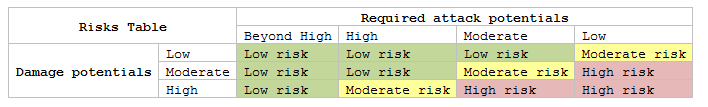
\includegraphics[width=\linewidth]{images/risktable.PNG} %  
		\caption{Risk Table}
        \label{tbl:risktable}
	\end{table}

\section{Document System Under Development}
\label{archdesign}
This section describes how the CliniScale project is modeled as a \textit{System Under Development (\textit{SUD})}. The applied process is defined in \textit{\nameref{moradocsud}} and results in the work product \textit{\nameref{morasud}}. Modeling the \textit{SUD} is essential to perform the security risk assessment as it describes the underlying system architecture. The \textit{SUD} is modeled after the process defined in \textit{\nameref{sysrequirements}}.


\subsection{Identify Functions}
\label{designIdFunc}

First step is to identify functions representing the main functionality of the CliniScale systems process. The process can be divided into three basic work steps: Configuration of the trial, performing the trial on selected probands and sending the trial results to the \textit{Trial Executor}. 

Configuration of the trial is the first process investigated. The \textit{Trial Executor}, the party that wants to create a clinical trial, and the \textit{Trial Configurator}, a service offered by the CliniScale project to create trials, take part in this process.\\
To model the first step of the process, the function "F.1: Create a clinical trial" is created.
This process is divided into two steps: The configuration of the trial and the communication of the configuration to CliniScale. 
To configure the trial, the \textit{Trial Executor} obtains the data needed from the \textit{Trial Configurator}. These include data such as forms to create surveys or lists of possible probands. \\
To represent this process, the sub-function "F.1.1: Configure clinical trial" is created.
Next step is to send the configured trial from the \textit{Trial Executor} to the \textit{Trial Configurator} service. The sub-function "F.1.2: Send trial configuration to the Trial Configurator" models this process.\\
\newline
To model the execution of the trial the function "F.2: Perform the trial" is created. This process is divided into three sub-processes: Communicating the trial to the probands mobile application, performing the trial by gathering the asked information and returning the collected information to the CliniScale back end.\\
"F.2.1: Send trial configuration to mobile application" represents the process of sending the trial configuration to the applications of selected probands. To model the execution of the trial the sub-function "F.2.2: Collect asked information" is created.
To represent the third sub-process, the sub-function "F.2.3: Return collected information to the CliniScale back end" is defined.\\
\newline
The last step of the process, the return of collected information to the \textit{Trial Executor}, is represented by the function "F.3: Report trial results". This function is divided into two sub-functions: "F.3.1: Bundle results" and "F.3.2: Send results to Trial Executor".\\
The first sub-function describes the process of creating a result report out of the collected information of the probands. The second sub-function models the communication of this report to the \textit{Trial Executor}.

\subsection{Define Components}
\label{designIdComp}
In order to define components, trust boundaries within the architecture have to be identified. Trust boundaries describe entity areas within the project where communication between components is assumed to be secure because communication never leaves the control of the operator of such trust boundary, whereas communication between components of different trust boundaries is mostly performed over the internet. This enables examination of the communication channels between components of different trust boundaries. These communication channels are the subject of research in this thesis, as the goal is to secure the communication between different parties.\\
\newline
First, the trust boundary representing the CliniScale environment and the components in it are defined. All components belonging to the CliniScale project itself are found within this boundary. A component called "Cmp.1: CS Environment", representing this trust boundary, is created. Within this component, two subcomponents representing the CliniScale back end and the \textit{Trial Configurator} are created: "Cmp.2: CS back end" and "Cmp.3: CS Trial Configurator".\\
\newline
The next trust boundary represents the proband using the CliniScale mobile application. The component "Cmp.4: Mobile Phone" is defined to model the trust boundary of the mobile device. This component consists of one subcomponent representing the CliniScale application: "Cmp.5: CS Application".\\
\newline
The third trust boundary describes the \textit{Trial Executor}. It is represented by the component "Cmp.6: Trial Executor". As how exactly this domain is structured is out of scope, since the \textit{Trial Executor} is an external party, no subcomponents can be specified.

\subsection{Define Data}
\label{designIdData}
Next step in modeling the \textit{SUD} is to define the data that is collected, processed and communicated in this project. Four different kinds of data are defined in \textit{\nameref{sysrequirements}}: HealthData, TrialConfig, TrialResults and ProbandData. For each a data element is created: "D.1: HealthData", "D.2: TrialConfig", "D.3: TrialResults" and "D.4: ProbandData". \\
\newline
"D.1: HealthData" describes gathered data of every proband in the process of executing the trial. These data may contain medical information, making it sensitive personal data according to the GDPR. "D.2: TrialConfig" models configuration of the clinical trial. Besides configuration of the trial, such as survey questions, specification of the time frame or scheduling, it also contains information about selected probands to perform the trial on. This information may not contain sensitive data of the probands, but it can enable linking of data to determine information compromising a probands right to self-determination. "D.3: TrialResults" bundles the trial results of every proband to be send to the \textit{Trial Executor}. It contains data concerning the health of participating probands and therefore is categorized as sensitive personal data. "D.4: ProbandData" models the information the \textit{Trial Configurator} communicates to the \textit{Trial Executor} to allow him to configure a clinical trial. It represents a set of probands the \textit{Trial Executor} can choose from to perform his trial on and therefore is declared sensitive information, as the disclosure can lead to the leak of various identities.\\
\newline
These data elements are assigned to the components that gather, process or store them in any step of the defined process. "D.1: HealthData" is assigned to "Cmp.2: CS Back end", "Cmp.5: CliniScale Application" and "Cmp.6: Trial Executor". "D.2: TrialConfiguration" is assigned to "Cmp.2: CS Back end". "D.3: TrialResults" is assigned to "Cmp.2: CS Back end" and "Cmp.6: Trial Executor". "D.4: ProbandData" is assigned to "Cmp.3: CS Trial Configurator" and "Cmp.6: Trial Executor".

\subsection{Define Communication Channels}
\label{designIdChannels}

The last task in the process of modeling the \textit{SUD} is to create channels between components to represent the communication between these. "Ch.1: Cmp.6(Trial Executor), Cmp.3(CS Trial Configurator)" models the communication between the \textit{Trial Executor} and the Trial Configurator. As it is a bidirectional communication, two data flows are created to represent both directions: "DF.1: D.4(ProbandData): Cmp.3(CS Trial Configurator) -> Cmp.6(Trial Executor)" and "DF.5: D.2(TrialConfiguration): \\Cmp.6(Trial Executor) -> Cmp.3(CS Trial Configurator)". The first data flow models the communication of "D.4: ProbandData" from the \textit{Trial Configurator} to the \textit{Trial Executor} to enable the configuration of the trial. The second data flow represents the communication of the data "D.2: TrialConfiguration" from the \textit{Trial Executor} to the \textit{Trial Configurator}.\\
\newline
"Ch.2: Cmp.2(CS back end), Cmp.5(CS Application)" models the communication between the CliniScale back end and the CliniScale mobile application. Two data flows represent the functionality of the channel. The first data flow, "DF.2: \\D.2(TrialConfiguration): Cmp.2(CS back end) -> Cmp.5(CS Application)", models the transport of "D.2: TrialConfig" from "Cmp.2: CS back end" to "Cmp.5: CS Application". "DF.3: D.1(HealthData): Cmp.5(CS Application) -> Cmp.2(CS back end)" models the other direction, transferring "D.1: HealthData" from "Cmp.5: Cs Application" to "Cmp.2: CS back end".\\
\newline
The last step to model the communication is to define the communication between "Cmp.2: CS back end" and "Cmp.6: Trial Executor" by creating the channel "Ch.3: Cmp.2(CS back end), Cmp.6(Trial Executor)". This channel consists of one data flow to represent the communication of "D.3: TrialResults" from "Cmp.2: CS back end" to "Cmp.6: Trial Executor": "DF.4: D.3(TrialResults): Cmp.2(CS back end) -> Cmp.6(Trial Executor)".\\
\newline
Figure \nameref{fig:sud} shows how the CliniScale system is modeled as \textit{SUD}.
\begin{figure}[H]
  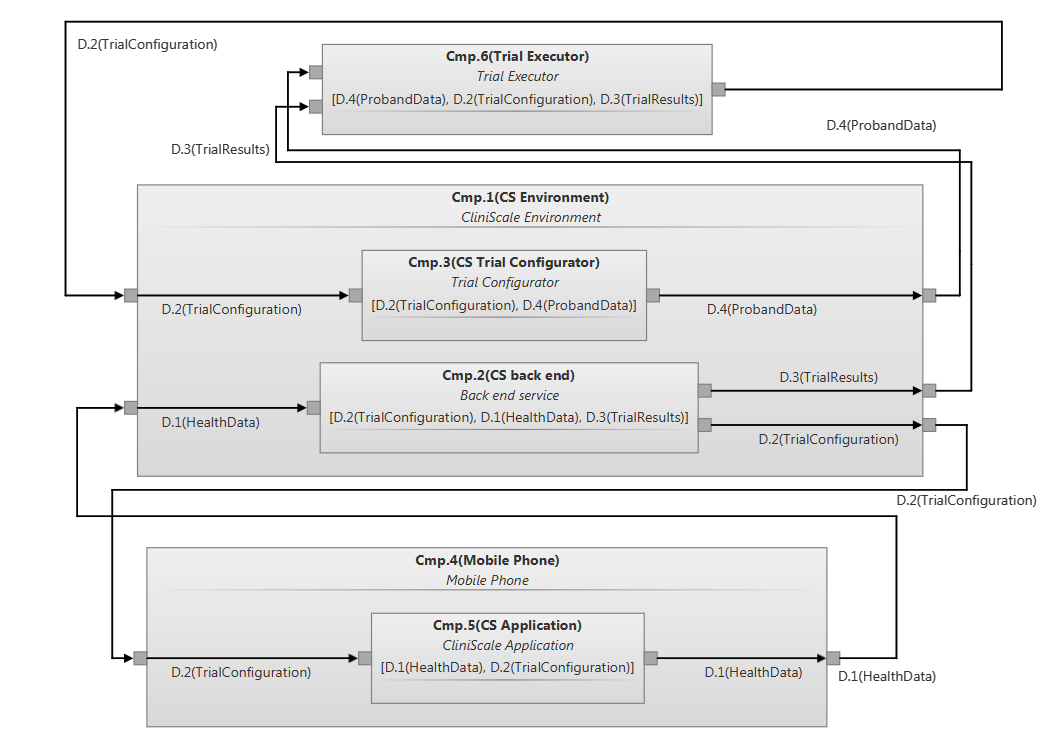
\includegraphics[width=1.4\linewidth, angle=90]{images/sud.png}
  \caption{System Under Development}
  \label{fig:sud}
\end{figure}

\subsection{Model the SUD in the Microsoft Threat Modeling Tool}
\label{SUDMTMT}
To use the Microsoft Threat Modeling Tool as a threat and control catalogue, the \textit{SUD} has to be modeled in it. 

First, three \textit{Generic Trust Boundaries} representing the \textit{CliniScale Environment}, the \textit{Trial Executor} and the mobile device running the \textit{CliniScale application} are created. These are named \textit{CliniScale Environment}, \textit{Trial Executor} and \textit{Mobile Device} representing respective components.
Next, a \textit{Web Application} and a \textit{Web API} are created inside the \textit{CliniScale Environment} trust boundary. The \textit{Web Application} is named \textit{TrialConfigurator} and the \textit{Web API} is named \textit{CliniScale back end} representing the components "Cmp.3: CS Trial Configurator" and "Cmp.2: CS back end".
To model the component "Cmp.5: CS Application" a \textit{Mobile Client} named \textit{CliniScale Application} is created inside the \textit{Mobile Device} trust boundary.
The \textit{Trial Executor} is represented as a \textit{Browser} inside the \textit{Trial Executor} trust boundary.

To model the channels and data flows between these components a pair of \textit{Request} and \textit{Response} elements is created for each data flow. The naming convention is "DF.X\_Request" for \textit{Request} elements and "DF.X\_[Data]" for the \textit{Response} elements containing the corresponding data. Five pairs of \textit{Request} and \textit{Response} elements are created in the process: "DF.1\_Request" and "DF.1\_ProbandData", "DF.2\_Request" and "DF.2\_TrialConfig", "DF.3\_Request" and "DF.3\_HealthData", "DF.4\_Request" and "DF.4\_TrialResults" and "DF.5\_Request" and "DF.5\_TrialConfig".
\\
Figure \ref{fig:mtmtmodel} shows the modeling of the \textit{SUD} in the Microsoft Threat Modeling Tool.
\begin{figure}[H]
  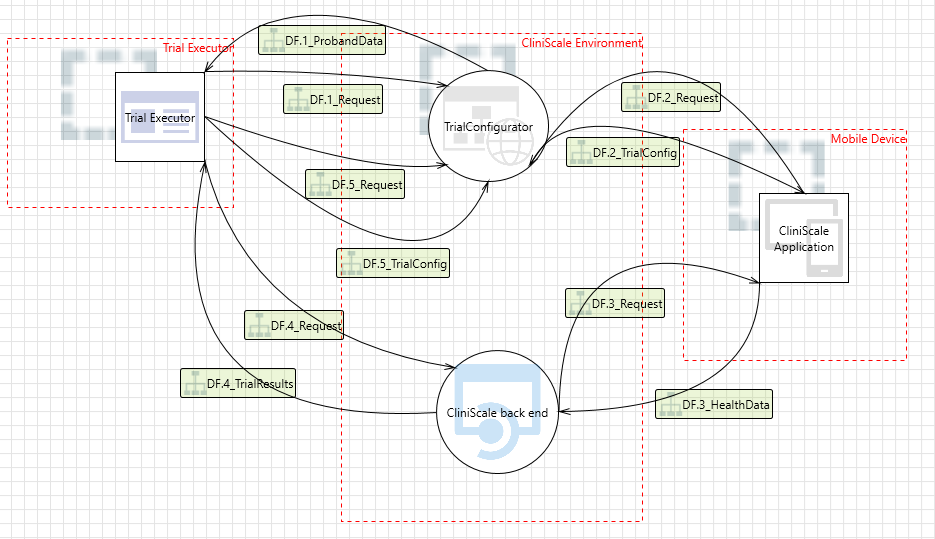
\includegraphics[width=\linewidth]{images/mtmt_model.PNG}
  \caption{Microsoft Threat Modeling Tool Model of the SUD}
  \label{fig:mtmtmodel}
\end{figure}


\subsection{Generate Threat and Control Catalogues}
This section describes how the Microsoft Threat Modeling Tool is used to generate threat and control catalogues applying to the \textit{SUD}.\\

The Microsoft Threat Modeling Tool automatically generates threats applying the \\STRIDE threat model. For the created model of the \textit{SUD}, 100 threats are generated. The generated threats contain this relevant information: name and description of the threat, STRIDE category, targeted element and possible mitigations.
\newline
The first step is to create the threat catalogue in the Yakindu Security Analyst. Six threat classes are created representing the STRIDE categories: "TC.1: Spoofing" targeting the security goal class "Authenticity", "TC.2: Tampering" targeting "Integrity", "TC.3: Repudiation" targeting "Accountability", "TC.4: Information disclosure" targeting "Confidentiality", "TC.5: Denial of Service" targeting "Availability" and "TC.6: Elevation of privilege" targeting "Authorization".
Next, a set of the exported list of generated Threats is created. The set includes 38 different threats which can be imported into the Yakindu Security Analyst as threat classes. The corresponding STRIDE category is set as refined threat class, e.g. "TC.4.1: An adversary can gain access to certain pages or the site as a whole." refines "TC.4: Information disclosure". The resulting threat catalogue consists of 44 threat classes.
\newline
The control catalogue is created in similar manner. First, control classes modeling the ten basic mitigation categories suggested by the Microsoft Threat Modeling Tool\cite{mtmtmitigations} are created: "CC.1: Auditing and Logging", "CC.2: Authentication", "CC.3: Authorization", "CC.4: Communication security", "CC.5: Configuration management", "CC.6: Cryptography", "CC.7: Exception management", "CC.8: Input validation", "CC.9: Sensitive Data" and "CC.10: Session management".
%ToDo: file verweis
\\
Next step is the creation of a set of suggested mitigations by the exported list of generated threats is created. This list consists of 72 suggested mitigations. These mitigations are imported as control classes. Each control class refines the corresponding mitigation category. The resulting control catalogue consists of 82 control classes.
%ToDo: file verweis

\section{Security Risk Assessment}
\label{riskassessment}
This section describes how the security risk assessment is performed following the process defined in \textit{\nameref{morachapter}}.


\subsection{Determine Protection Needs}
As the goal of the security risk analysis is to secure communications within the CliniScale project, the creation of security goals focuses on data and data flow elements.\\
First step is to create a set of security goals for every data flow element. Using the \textit{Security Goal Assessment} of the Yakindu Security Analyst, a security goal for every security goal class can be generated for every data flow element. In the process 30 security goals targeting the corresponding data flow element are created.\\
The same procedure is repeated to create security goals for every data element, resulting in 24 more security goals. The generated security goals for data elements get assigned a depends on relation to every security goal concerning a data flow transferring matching data and matching security goal class, e.g. the security goal "G.43: Confidentiality TrialResults" depends on "G.19: Confidentiality D.3(TrialResults): \\Cmp.2(CS back end) -> Cmp.6(Trial Executor)".
\newline
Next step is to determine damage criteria for the generated security goals. This procedure defines a damage potential for every security goal in order to estimate arising risks in case of a breach of the security properties. It creates compliance with the requirement of the GDPR to implement security measures appropriate to the risks in case of a loss of security properties. First, the damage criteria for security goals concerning data elements are set. As these security goals have a depends on relation to the security goals concerning data flows transferring the data, the damage potential defined by the assigned damage criteria is propagated towards the data flows security goals.\\
\newline
"D.1: HealthData" is a critical data element, as a leak of the data would breach the GDPR and have existence threatening fines and reputational damage as consequence. Therefore, the security goal concerning confidentiality, "G.31: Confidentiality HealthData", is assigned with the damage criteria "Existence-threatening fine" and "Existence-threatening reputational damage". As sensible personal data is leaked to non-authorized parties, the damage criterion "Leak of sensitive personal data" is also assigned. Availability of "D.1: HealthData" induces contract breaches resulting in fines, resulting in "Considerable fine" being assigned as damage criterion. Lacking integrity of "D.1: HealthData" can lead to breach of contract with companies performing clinical trials with CliniScale, resulting in fines and damaged reputation. Accordingly, the damage criteria "Considerable fine" and "Negligible reputational damage" are assigned. Breach of authenticity can lead to a loss of confidentiality of "D.1: HealthData". Because of this, "G.31: Confidentiality HealthData" is set in a depends on relation with "G.34: Authenticity HealthData", leading to a propagation of the damage potential towards the authenticity security goal. Accountability has a minor impact on "D.1: HealthData" regarding contracts, therefore the damage criterion "Negligible fine" is assigned. Lack of authorization leads to a loss of confidentiality, so "G.36: Authorization HealthData" is added to the depends on relation of "G.31: Confidentiality HealthData" inheriting its damage potential.\\
\newline
The data element "D.2: TrialConfiguration" is critical to perform a clinical trial. \\Breaches to its security goals can lead to substantial fines and reputational damage. As "D.2: TrialConfiguration" also contains identities of possible probands, there is a risk of leaking various identities, having a grave impact on the reputation of the CliniScale project. Breach of confidentiality leads to these consequences. Therefore, the damage criteria "Considerable fine", "Existence-threatening reputational damage" and "Leak of multiple identities" are assigned to the security goal "G.37: Confidentiality TrialConfiguration". Lacking availability leads to breaches of contract and minor reputational damage, as customers might want to choose a competitor when performing their next clinical trial. "G.38 Availability TrialConfiguration" is assigned with the damage criteria "Negligible fine" and "Negligible reputational damage". Integrity of the data is essential to perform a clinical trial and a breach can lead to substantial contract breaches. Therefore, the damage criteria "Considerable fine" and "Negligible reputational damage" are assigned. Breaches of authenticity and authorization lead to a loss of confidentiality. Both "G.40: Authenticity TrialConfiguration" and "G.42: Authorization TrialConfiguration" are added to the depends on relation of "G.37: Confidentiality TrialConfiguration". Lack of accountability may lead to minor fines due to contract breaches, so the damage criterion "Negligible fine" is assigned to "G.41: Accountability TrialConfiguration".\\
\newline
"D.3: TrialResults" contains sensitive personal data and a breach can lead to a leak of multiple identities. Fines by the GDPR and with it, major reputational damage, are possible. Therefore, "G.43: Confidentiality TrialResults" is a critical security goal assigned with the damage criteria "Existence-threatening fine", "Existence-threatening reputational damage", "Leak of sensitive personal data" and "Leak of multiple identities". Availability of the data is important to keep up with signed contracts. "Considerable fine" and "Considerable reputational damage" are assigned to "G.44: Availability TrialResults" as consequence. A breach of integrity can lead to falsified results of the clinical trial resulting in major contract breaches. Therefore "Considerable fine" and "Considerable reputational damage" are assigned to "G.45: Integrity TrialResults". Authorization and authenticity of the investigated element lead to a loss of confidentiality, therefore both security goals are added to the depends on relation of "G.43: Confidentiality TrialResults". Breach of accountability can lead to contract breaches resulting in considerable fines. "Considerable fine" is assigned as damage criterion to "G.47: Accountability TrialResults".\\
\newline
The data element "D.4: ProbandData" consists of various identities of possible \\probands. A breach to its security goals leads to fines defined in the GDPR, leak of multiple identities and major reputational damage. Confidentiality is a critical security property. The damage criteria "Considerable fine", "Considerable reputational damage" and "Leak of multiple identities" are assigned to "G.49: Confidentiality ProbandData". Lack of availability of "D.4: ProbandData" can lead to a delay of the trial and minor contract breaches due to missing service standards. Therefore, "Negligible fine" is assigned to "G.50: Availability ProbandData". Missing integrity of the data can lead to probands being chosen for a study without being qualified. This can lead to considerable contract breaches and some reputational damage. The damage criteria "Considerable fine" and "Negligible reputational damage" are assigned to "G.51: Integrity ProbandData". Lack of authorization and authenticity leads to a breach towards confidentiality, therefore "G.52: Authenticity ProbandData" and "G.54: Authorization ProbandData" are assigned to "G.49: Confidentiality ProbandData" in a depends on relation. A breach of accountability can lead to minor contract breaches. "Negligible fine" is added to "G.53: Accountability ProbandData"\\
\newline
Security goals for data flows are investigated next. As the security goals for the transported data are already defined, every security goal concerning a data flow is set in a depends on relation with the matching security goal for the data element and security goal class, e.g. the security goal concerning confidentiality of ”DF.1: D.4(ProbandData): Cmp.3(CS Trial Configurator) -> Cmp.6(Trial Executor)”, "G.1: Confidentiality D.4(ProbandData): Cmp.3(CS Trial Configurator) -> Cmp.6(Trial Executor)” is assigned into the depends on relation of "G.49: Confidentiality ProbandData".\\
\newline
In the process, 54 security goals have been created, 30 security goals concerning data flow elements and 24 security goals concerning data elements. 27 of the security goals have a damage potential "High", 15 a damage potential of "Moderate" and twelve the damage potential "Low".


\subsection{Analyze Threats}
A threat is created for every threat class, except the threat classes modeling the STRIDE categories. In the process, 38 threats are created.\\
To identify the security goals every threat threatens, the exported list of generated threats by the Microsoft Threat Modeling Tool is searched for appearances of every threat to identify the threatened architecture element. By matching the STRIDE category, the corresponding security goal is found.\\
\newline
First, threats of the STRIDE category "Spoofing" are investigated. The first threat "T.1: Create fake website to phish" instantiates the threat class "TC.1.1". The identified security goals threatened are "G.4", "G.10" and "G.28". "T.2: Gain access to API end points due to unrestricted cross domain requests" instantiates "TC.1.2" and threatens the security goal "G.22". The third threat, "T.3: Gain access to user's session due to improper logout", instantiates "TC.1.3" and threatens "G.4" and "G.28". The threats "T.4: Spoof targets Web Application due to insecure TLS certificate configuration" and "T.5: Steal sensitive data like user credentials" both threaten "G.4", "G.10" and "G.28". "T.4" instantiates "TC.1.4" and "T.5" "TC.1.5". "T.6: Spoof browser and gain access to Web API" instantiates "TC.1.6" and threatens "G.22". The threat "T.7: Obtain refresh/access tokens and gain access to API" instantiating "TC.1.7" threatens "G.16". The threats "T.8: Steal session cookies due to bad attributes", instantiating "TC.1.8", "T.9: Gain access to a user's session due to insecure coding practices", instantiating "TC.1.9", and "T.10: Spoof browser to gain access to Web Application", instantiating "TC.1.10", all threaten the security goals "G.4" and "G.28". "T.11: Spoof Mobile client to gain access to Web API" threatens "G.16" and instantiates "TC.1.11". The last threat of the category "Spoofing" is "T.12: Spoof Mobile client to gain access to Web Application" and instantiates "TC.1.12". It threatens "G.10". \\
\newline
Next step is to create threats of the category "Tampering". "T.13: Deface target web application by injecting malicious code or uploading dangerous files" instantiates "TC.2.1" and targets "G.3" and "G.27". The threat "T.14: SQL injection through Web API" instantiates "TC.2.2" and threatens "G.15" and "G.21". "T.15: Reverse engineer and tamper binaries" targets "G.9" and "G.15" and is an instance of "TC.2.3". "TC.2.4" is instantiated by "T.16: Inject malicious input into API and affect downstream processes". The threat targets "G.15" and "G.21". "T.17: Replay attacks" instantiates "TC.2.5" and targets "G.9" and "G.27". The threats "T.18: SQL injection through Web API" and "T.19: Access sensitive data stored in Web App's config files" instantiate "TC.2.6" and "TC.2.7" respectively and target "G.2", "G.9" and "G.27".\\
\newline
Following presents threats of the category "Repudiation". "T.20: Deny malicious act on API" instantiates "TC.3.1" and threatens "G.17" and "G.23". The threat "T21: Remove attack foot prints" targets "G.5", "G.11" and "G.29". It instantiates the threat class "TC.3.2".\\
\newline
Next, threats representing the "Information disclosure" category of STRIDE are created. "T.22: Gain access to certain pages or hole site" instantiates "TC.4.1" and threatens "G.1" and "G.25". The threat "T.23: Sniff traffic from Mobile client" instantiates "TC.4.2" and targets "G.7" and "G.13". "T.24: Access sensitive data stored in config files" is an instance of "TC.4.3" and threatens "G.13" and "G.19". "T.25: Access sensitive information through error messages" instantiating "TC.4.4", "T.27: Reverse weakly encrypted/hashed content" instantiating "TC.4.6" and the instance of "TC.4.7", "T.28: Access sensitive data from log files" all threaten "G.1", "G.7" and "G.25". "T.26: Gain sensitive data from mobile device" instantiates "TC.4.5" and threatens "G.7" and "G.13". The threat "T.29: Access sensitive data from uncleared browser cache" is an instance of "TC.4.8" and targets "G.1" and "G.25". "T.30: Access unmasked sensitive data" is an instance of "TC.4.9" and threatens "G.1" and "G.25". The threat "T.31: Retrieve sensitive data from browser storage" instantiates "TC.4.10" and targets "G.19". Both threats "T.32: Sniff traffic to the Web API", instance of "TC.4.11", and "T.34: Access sensitive information through error messages from API", instantiating "TC.4.13" threaten "G.13" and "G.19". "T.33: Sniff traffic to Web Application" is an instance of "TC.4.12" and threatens "G.2" and "G.25".\\
\newline
"Denial of service" is the next category of created threats. The only threat of this category, "T.35: Lack of controls against cross domain requests", is an instance of "TC.5.1" and threatens "G.2" and "G.26".\\
\newline
Next are threats of the STRIDE category "Elevation of privileges". "T.36: Improper validation logic" instantiates "TC.6.1" and threatens "G.6" and "G.30". The threat "T.37: Access Web API due to poor access control checks", instance of "TC.6.2", targets "G.18" and "G.24". The threat "T.38: Jailbreak mobile phone" is an instance of "TC.6.3" and threatens "G.12" and "G.18".\\
\newline

\subsection{Analyze Risks}
\label{ReqAssARisks}
To define risks, a risk element is created for every threat defined and the threat is assigned to it using the "caused by" relation. Based on the defined calculation in the Assessment Model, the risk level for every risk element is computed by using the required attack potential of the assigned threat and the damage potential of threatened security goals. \\
In the process, 38 risk elements are defined. Figure \ref{fig:bubblechart} shows a bubble chart displaying the partition of risk levels on the defined risk elements. As the overall risk level is too high for being acceptable as a security concept, controls have to be established to diminish the effects of identified threats.

\begin{figure}[H]
  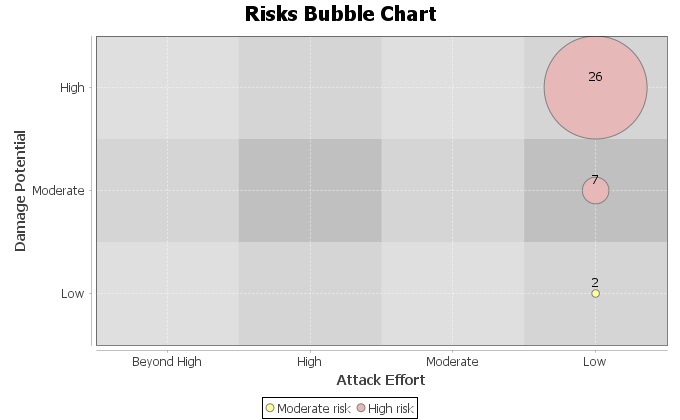
\includegraphics[width=\linewidth]{images/bubble_p1.png}
  \caption{Risk Bubble Chart}
  \label{fig:bubblechart}
\end{figure}


\subsection{Establish Controls}
Similar to threats, a control is created for every entry in the threat catalogue except the ten main control classes of the Microsoft Threat Modeling Tool. Mitigated threats are identified by inspecting every threat’s suggested mitigations. If it contains the current investigated control class, the threat is mitigated by it.\\
\newline
First, controls of the category "Auditing and Logging" are investigated. The first control is "C.1: Ensure that auditing and logging is enforced on Web API", instantiating "CC.1.1" and mitigating "T.20". The controls "C.2: Ensure that log rotation and separation are in place", instantiating "CC.1.2", "C.5: Ensure that User Management Events are Logged", instantiating "CC.1.5", and "C.6: Ensure that auditing and logging is enforced on the application", instantiating ""CC.1.6" mitigate "T.21". "C.3: Ensure that the application does not log sensitive user data" mitigates "T.28" and is an instance of "CC.1.3". "T.28" and "T.21" are mitigated by the control "C.4: Ensure that Audit and Log Files have Restricted Access", an instance of "CC.1.4". The last control of this category, "C.7: Ensure that the system has inbuilt defences against misuse", is an instance of "CC.1.7" and mitigates "T.13". \\
\newline
Next, controls of the category "Authentication" are identified. "C.8: Consider using a standard authentication mechanism to authenticate to Web Application" is an instance of "CC.2.1" and diminishes the threats "T.10" and "T.12". The usage of proven cryptographic methods enables setting the required attack potential to "Beyond High". The controls "C.9: Enable step up or adaptive authentication", instance of "CC.2.2", "C.11: Implement forgot password functionalities securely", instance of "CC.2.4", and "C.12: Ensure that password and account policy are implemented", instance of "CC.2.5", all ease the effects of "T.5". "C.10: Ensure that administrative interfaces are appropriately locked down" instantiates "CC.2.3" and mitigates the effects of the threats "T.22" and "T.36". The control "C.13: Implement controls to prevent username enumeration" instantiates "CC.2.6" and mitigates "T.25". "T.6" and "T.11" are mitigated by an instance of "CC.2.7", "C.14: Ensure that standard authentication techniques are used to secure Web APIs". As cryptographic standards can be used, providing proven security mechanisms, the required attack potential is set to "Beyond High". The control "C.15: Use ADAL libraries to manage token requests from OAuth2 clients to AAD" eases the effects of "T.7". It is an instance of "CC.2.8". \\
\newline
The third category of controls that are investigated is "Authorization". "C.16: Enforce sequential step order when processing business logic flows", "C.17: Ensure that proper authorization is in place and principle of least privileges is followed", "C.18: Business logic and resource access authorization decisions should not be based on incoming request parameters" and "C.19: Ensure that content and resources are not enumerable or accessible via forceful browsing" all mitigate the effects of "T.36". They are instances of, in order, "CC.3.1", "CC.3.2", "CC.3.3" and "CC.3.4". The control "C.20: Implement implicit jailbreak or rooting detection" is an instance of "CC.3.5". It reduces the effects of "T.38". "C.21: Implement proper authorization mechanism in ASP.NET Web API" is an instance of "CC.3.6". The required attack potential is set to "Beyond High", as modern cryptography standards are used. It mitigates the threat "T.37". \\
\newline
Next, the category "Communication Security" is investigated. Since it applies the use of proven cryptographic standards on communication, the required attack potential of its controls is set to "Beyond High" as default value. "C.22: Verify X.509 certificates used to authenticate SSL, TLS, and DTLS connections" is an instance of "CC.4.1" and mitigates the threats "T.1", "T.4" and "T.27". The control "C.23: Enable HTTP Strict Transport Security (HSTS)" instantiates "CC.4.2" and mitigates the effects of "T.13" and "T.33". "C.24: Implement Certificate Pinning" instances "CC.4.3" and mitigates "T.23". Last control of the category is "C.25: Force all traffic to Web APIs over HTTPS connection". It's an instance of "CC.4.4" and diminishes the effects of "T.17" and "T.32".\\ 
\newline
"Configuration Management" is the next category proposed by the Microsoft Threat Modeling Tool that is investigated. "C.26: Implement Content Security Policy (CSP), and disable inline javascript" and "C.27: Enable browser's XSS filter" are instances of "CC.5.1" and "CC.5.2" respectively. They mitigate the threat "T.13". The control "C.28: ASP.NET applications must disable tracing and debugging prior to deployment" mitigates "T.25" and is an instance of "CC.5.3". "C.29: Ensure that only trusted origins are allowed if CORS is enabled on ASP.NET Web Applications" instances "CC.5.4" and mitigates the threats "T.2" and "T.35". "C.30: Enable ValidateRequest attribute on ASP.NET Pages" is an instance of "CC.5.5" and mitigates "T.9" and "T.13". The controls "C.31: Use locally-hosted latest versions of JavaScript libraries", instance of "CC.5.6", "C.32: Disable automatic MIME sniffing", instance of "CC.5.7", and "C.35: Access third party javascripts from trusted sources only", instance of "CC.5.10", all mitigate "T.13". "C.33: Encrypt sections of Web API's configuration files that contain sensitive data" is an instance of "CC.5.8" and mitigates "T.24". The control "C.34: Ensure authenticated ASP.NET pages incorporate UI Redressing" diminishes the effects of "T.1" and "T.35". It instantiates of "CC.5.9".\\
\newline
The next investigated category is "Cryptography". The required attack potential of controls of this category is set to "Beyond High", as they all propose the implementation of cryptographic standards with proven security levels. The seven controls of this category all mitigate "T.27". They define the use of cryptographic standards and their configuration. "CC.6.1" is instantiated by "C.36: Use only approved symmetric block ciphers and key lengths". "C.37: Use approved block cipher modes and initialization vectors for symmetric ciphers" instantiates "CC.6.2". "C.38: Use approved asymmetric algorithms, key lengths, and padding" is an instance of "CC.6.3". "CC.6.4" is instantiated by the control "C.39: Use approved random number generators". The control "C.40: Do not use symmetric stream ciphers" instantiates "CC.6.5". "C.41: Use approved MAC/HMAC/keyed hash algorithms" instantiates "CC.6.6". The last control of this category, "C.42: Use only approved cryptographic hash functions" is an instance of "CC.6.7". \\
\newline
"Exception Management" is the seventh category where controls are identified. "C.43: Ensure that proper exception handling is done in ASP.NET Web API" instantiates "CC.7.1" and mitigates "T.34". "T.25" and "T.27" are mitigated by the controls "C.44: Do not expose security details in error messages", "C.45: Implement Default error handling page" and "C.46: Set Deployment Method to Retail in IIS". They represent instances of "CC.7.2", "CC.7.3" and "CC.7.4" respectively. "C.47: Exceptions should fail safely" instantiates "CC.7.5" and helps mitigating "T.25".\\
\newline
The next category of controls investigated is "Input Validation". "C.48: Ensure that each page that could contain user controllable content opts out of automatic MIME sniffing", instance of "CC.8.1", and "C.49: Ensure appropriate controls are in place when accepting files from users", instance of "CC.8.2", both mitigate the effect of threat "T.13". The control "C.50: Ensure that type-safe parameters are used in Web Application for data access" instantiates "CC.8.3" and mitigates "T.18". The controls "C.51: Encode untrusted web output prior to rendering", "C.53: Do not assign DOM elements to sinks that do not have inbuilt encoding" and "C.56: Avoid using Html.Raw in Razor views" all diminish the effects of "T.9" and "T.13". They instantiate "CC.8.4", "CC.8.6" and "CC.8.9" respectively. "C.52: Perform input validation and filtering on all string type Model properties" is an instance of "CC.8.5" and "C.55: Implement input validation on all string type parameters accepted by Controller methods" an instance of "CC.8.8". Both mitigate the effects of "T.5" and "T.13". "C.54: Validate all redirects within the application are closed or done safely" is an instance of "CC.8.7" and mitigates the threats "T.1" and "T.5". "C.57: Ensure that model validation is done on Web API methods", instance of \\"CC.8.10", and "C.58: Implement input validation on all string type parameters accepted by Web API methods", instance of "CC.8.11", both mitigate "T.16". The control "C.59: Ensure that type-safe parameters are used in Web API for data access", instance of "CC.8.12", eases the effects of "T.14". The last control of the category is "C.60: Sanitization should be applied on form fields that accept all characters such as rich text editor". It's an instance of "CC.8.13" and mitigates "T.9" and "T.13".\\ 
\newline
The ninth category of controls proposed by the Microsoft Threat Modeling Tool is "Sensitive Data". "C.61: Ensure that sensitive content is not cached on the browser" is an instance of "CC.9.1" and mitigates the threat "T.29". The control "C.62: Encrypt sections of Web App's configuration files that contain sensitive data" is an instance of "CC.9.2". Due to the security level of applied encryption, the required attack potential is set to "Beyond High". It mitigates the effect of "T.19". "C.63: Explicitly disable the autocomplete HTML attribute in sensitive forms and inputs" instantiates "CC.9.3" and mitigates "T.5". The control "C.64: Ensure that sensitive data displayed on the user screen is masked" diminishes the threats of "T.30". It's an instance of "CC.9.4". "CC.9.5" is instantiated by "C.65: Ensure that sensitive data relevant to Web API is not stored in browser's storage". This control mitigates "T.31". "C.66: Encrypt sensitive or PII data written to phones local storage" is an instance of "CC.9.6" and mitigates "T.26". The controls required attack potential is raised to "Beyond High" due to the nature of enforced cryptographic methods. "C.67: Obfuscate generated binaries before distributing to end users" mitigates "T.15" and instantiates "CC.9.7". \\
\newline
The last category of controls is "Session Management". "C.68: Applications available over HTTPS must use secure cookies" is an instance of "CC.10.1" and diminishes the effects of "T.8" and "T.33". The control "C.69: All http based application should specify http only for cookie definition" is an instance of "CC.10.2" and mitigates "T.8". "C.70: Mitigate against Cross-Site Request Forgery (CSRF) attacks on ASP.NET web pages" mitigates the threats "T.2" and "T.35". It's an instance of "CC.10.3". The controls "C.71: Set up session for inactivity lifetime", instance of "CC.10.4", and "C.72: Implement proper logout from the application", instance of "CC.10.5", both mitigate "T.3". 


\subsection{Analyze Need for Further Iterations}

The effects of the controls on their mitigated threats is computed by the Yakindu Security Analyst. The risks created in \textit{\nameref{ReqAssARisks}} compute a new risk level for every risk as shown in Figure \ref{fig:bubblechart_p2}.

\begin{figure}[H]
  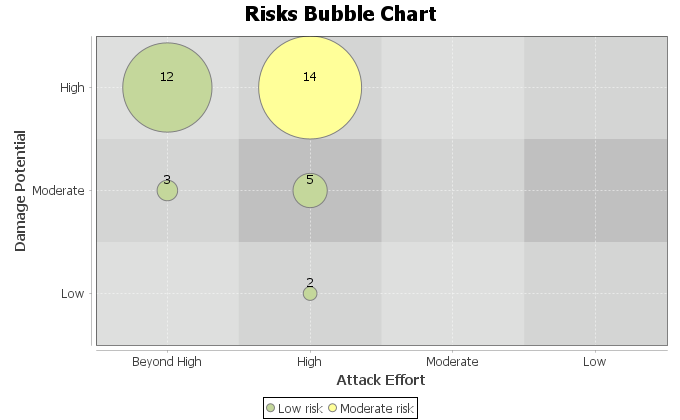
\includegraphics[width=\linewidth]{images/bubble_p2.png}
  \caption{Final Risk Bubble Chart}
  \label{fig:bubblechart_p2}
\end{figure}

15 of the risks have a risk level of "Moderate" and 23 a risk level of "Low". This is acceptable as an overall risk level.\\
Still, some of the identified controls introduce new elements to the \textit{SUD} needed for their implementation. Specifically, controls that implement cryptographic protocols, such as "C.25", need a secure storage to save cryptographic keys. To model these new components, the \textit{SUD} is altered by creating three new components: "Cmp.7: Secure Storage (CliniScale)", "Cmp.8: Secure Storage (Mobile Device)" and "Cmp.9: Secure Storage (Trial Executor)". New data elements modeling the public and secret keys saved in each storage are defined: "D.5: Public Key CliniScale", "D.6: Private Key CliniScale", "D.7: Public Key Trial Executor", "D.8: Private Key Trial Executor", "D.9: Public Key Mobile Device" and "D.10: Private Key Mobile Device". \\
Next, the defined data elements are assigned to the storage elements. Each storage element contains the public and private key corresponding to his party and the public keys of every party there is a connection to. "Cmp.7: Secure storage (CliniScale)" stores "D.5: Public Key CliniScale", "D.6: Private Key CliniScale", "D.7: Public Key Trial Executor" and "D.9: Public Key Mobile Device". "Cmp.8: Secure Storage (Mobile Device)" stores "D.5: Public Key CliniScale", "D.9: Public Key Mobile Device" and "D.10: Private Key Mobile Device". "Cmp.9: Secure Storage (Trial Executor)" stores "D.5: Public Key CliniScale", "D.7: Public Key Trial Executor" and "D.8: Private Key Trial Executor".\\
\newline

\begin{figure}
  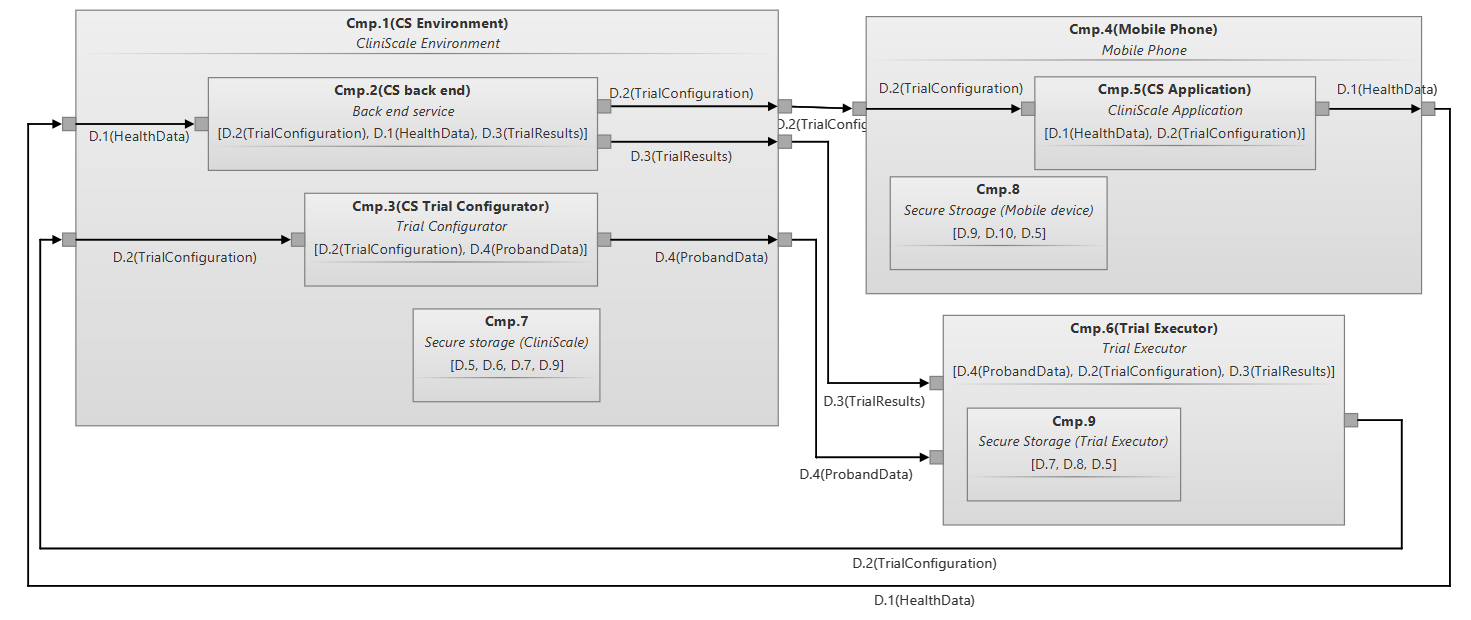
\includegraphics[width=1.4\linewidth, angle=90]{images/phase2.png}
  \caption{Updated SUD}
  \label{fig:phase2}
\end{figure}

Figure \ref{fig:phase2} shows the updated \textit{SUD}. As the scope of this thesis is securing the transfer of data and there is no new data flow introduced, the security risk assessment is therefore completed at this point.




